\chapter{Model improvements}


\section{Feature Engineering}
In order to improve our model performances, we focused our attention on feature engineering. Specifically we tried to extract stylometric, structural, orientation and vocabulary based features\cite{features}. Apart from this we also generated a word embedding vector of the words contained in each song's lyric by using SpaCy's\cite{spacy} pre-trained language model based on word2vec\cite{word2vec}.\par

Here is a comprehensive list of the features we extracted from our dataset, followed by a brief description:

\begin{description}
\item \textbf{Title\_vector}: word embedding vector of the song's title
\item \textbf{Lyric\_vector}: word embedding vector of the lyric content
\item \textbf{\%Rhymes}: defined as the percentage of the number of rhymes over the number of total lines. A rhyme is defined as a rhyme between two following lines
\item \textbf{Line\_count}: number of lines in the lyric
\item \textbf{Word\_count}: number of words in the lyric
\item \textbf{\%Past\_tense\_verbs}: defined as the the percentage of the number of past tense verbs over the total number of verbs
\item \textbf{\%Present\_tense\_verbs}: defined as the the percentage of the number of present tense verbs over the total number of verbs
\item \textbf{\%Future\_tense\_verbs}: defined as the the percentage of the number of future tense verbs over the total number of verbs, where future is just will + base form
\item \textbf{\%ADJ}: percentage of adjectives over the total number of words
\item \textbf{\%ADP}: percentage of adpositions (e.g. in, to, during) over the total number of words
\item \textbf{\%ADV}: percentage of adverbs (e.g. very, tomorrow, down, where, there) over the total number of words
\item \textbf{\%AUX}: percentage of auxiliaries (e.g. is, has (done), will (do), should (do)) over the total number of words
\item \textbf{\%INTJ}: percentage of interjections (e.g. psst, ouch, bravo, hello) over the total number of words
\item \textbf{\%NOUN}: percentage of nouns over the total number of words
\item \textbf{\%NUM}: percentage of numerals over the total number of words
\item \textbf{\%PRON}: percentage of pronouns (e.g. I, you, he, she, myself, themselves, somebody,...) over the total number of words
\item \textbf{\%PROPN}: percentage of proper nouns (e.g. Mary, John) over the total number of words
\item \textbf{\%PUNCT}: percentage of puntuctuation (e.g. ., (, ), ?) over the total number of words
\item \textbf{\%VERB}: percentage of verbs over the total number of words
\item \textbf{Selfish\_degree}: percentage of 'I' pronouns over the total number of pronouns
\item \textbf{\%Echoism}: percentage of echoism over the total number of words, where an echoism is either a sequence of two subsequent repeated words or the repetition of a vowel in a word
\item \textbf{\%Duplicate\_Lines}: number of lines duplicated across the lyric text
\item \textbf{isTitleInLyric}: boolean, true if the title string is also a substring of the lyric
\item \textbf{Sentiment}: sentiment between -1 and 1
\item \textbf{Subjectivity\_degree}: degree of subjectivity of the text
\end{description}

Since the word embedding vectors we generated had length 300, at the end we were able to obtain 623 distinct numerical features for each of the songs in our dataset.

\subsection{Feature Selection}

Having to deal with 623 different features for discriminating songs among 4 classes is probably enough and many features may be redundant or may not bring any useful information to our goal. Indeed, after running many experiments, we tried to keep our models as simple as possible by trying to select the fewer number of features possible.

In the end, we obtained the best results just by using the following features: \textit{Lyric\_vector}, \textit{\%Echoisms}, \textit{\%Duplicate\_Lines}, \textit{isTitleInLyrc}, \textit{\%Past\_tense\_verbs}, \textit{\%Present\_tense\_verbs}, \textit{\%Future\_tense\_verbs}, \textit{\%ADJ}, \textit{\%PUNCT}, \textit{Sentiment} and \textit{Subjectivity\_degree}. This process of feature selection left us with just 310 distinct features per song.


\section{MoodyLyrics duplicates bug}
During the analysis of MoodyLyrics described in the previous chapter we detected the presence of duplicated songs inside the dataset. Moreover, sometimes different emotions were associated with the duplicated songs. Thus, to continue our analysis we eliminated duplicated rows and we chose as emotion label the most frequent emotion between all the duplicates.\par
After reporting the bug to MoodyLyrics owners we have been suggested to use MoodyLyrics4Q, that, according to the creators is a more accurate version of MoodyLyrics.\par
This advice opened us three possibilities: continue using MoodyLyrics, start using MoodyLyrics4Q or create a new dataset as the concatenation of the previous two. We decided to start using all these three models, in order to understand which one, at the end, will give us a better playlists classification. The complete MoodyLyrics emotion classification analysis can be found at \href{https://github.com/sgiammy/emotion-patterns-in-music-playlists/blob/master/Notebook/1_ED_in_songs_lyrics.ipynb}{Notebook 1} while the MoodyLyrics4Q and the emotion detection analysis in the merged datasets can be found at \href{https://github.com/sgiammy/emotion-patterns-in-music-playlists/blob/master/Notebook/2_Advanced_Feature_Engineering.ipynb}{Notebook 2}.


\section{MoodyLyrics4Q}
MoodyLyrics4Q contains 2000 songs and has the same annotation schema as MoodyLyrics. Fig \ref{fig:stats}
shows the emotions distribution comparison between the two MoodyLyrics versions.

\begin{figure}[H]
\centering
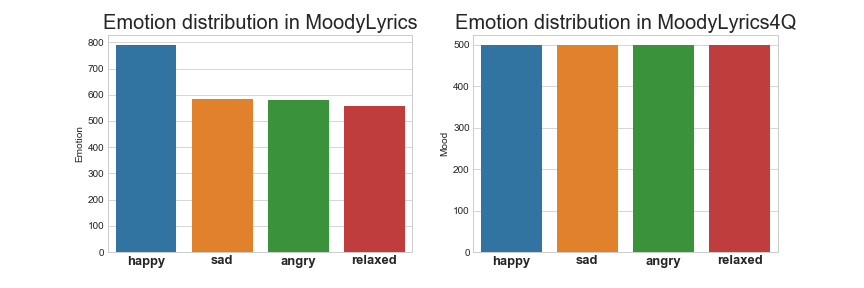
\includegraphics[width=1.1\textwidth]{./chapters/chapter5/images/Stats.png}
\caption{Emotions distribution comparison between MoodyLyrics and MoodyLyrics4Q}
\label{fig:stats}
\end{figure}

MoodyLyrics4Q classes are more much balanced, however MoodyLyrics4Q contains only 2000 songs instead of 2509. \par
We studied the qualitative difference between the two version comparing the classification given to the songs contained in both datasets to establish what version, according to us, is more correct. The intersection between the two versions contains 47 songs, and 21 over 47 have been classified differently. We noticed that in 15 over this 21 songs the two datasets confuses \textit{happy} with \textit{relaxed} and \textit{angry} with \textit{sad}. Indeed, only 6 of 21 songs are classified totally differently, however reading the lyrics of each of this song we could not establish which version is the best one.



\section{Results}
In this section we present the result obtained while predicting one of the four emotion labels \textit{relaxed}, \textit{happy}, \textit{sad}, \textit{angry}, using an artificial neural network, a support vector machine, the logistic regression and xgboost. The accuracies have been computed with a 5-fold cross validation. All the implementation details can be found at \href{https://github.com/sgiammy/emotion-patterns-in-music-playlists/blob/master/Notebook/2_Advanced_Feature_Engineering.ipynb}{Notebook 2}.

\begin{table}[H]
\begin{tabular}{ |p{3cm}||p{1.5cm}|p{1.5cm}|p{1.5cm}|p{1.5cm}|  }
 \hline
 \multicolumn{5}{|c|}{5-fold Cross Validation Accuracy} \\
 \hline
 Dataset & ANN & LR &SVM & xgboost\\
 \hline
MoodyLyrics4Q  & 51\%    &55\% &  59\% & 56\%\\
Both together &   67\%  & 68\%   &69\% &63.7\%\\
\hline
\end{tabular}
\caption{Emotion detection accuracies} \label{tab:comparison}
\end{table}

\begin{figure}[H]
  \centering
  \begin{subfigure}[b]{0.49\linewidth}
    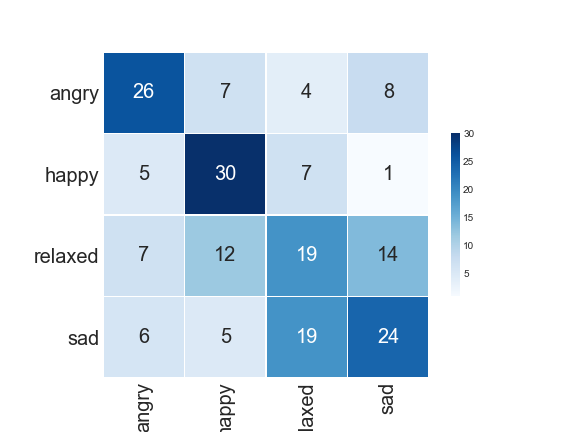
\includegraphics[width=\linewidth]{./chapters/chapter5/images/4Q/CM_ANN.png}
    \caption{ML4Q}
  \end{subfigure}
  \begin{subfigure}[b]{0.49\linewidth}
   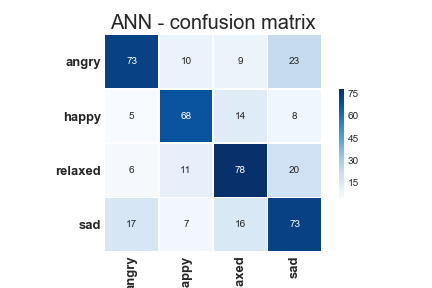
\includegraphics[width=\linewidth]{./chapters/chapter5/images/join/CM_ANN.png}
    \caption{ML + ML4Q}
  \end{subfigure}
  \caption{Artificial Neural Network - Confusion Matrix}
  \label{fig:ann}
\end{figure}

\begin{figure}[H]
  \centering
  \begin{subfigure}[b]{0.49\linewidth}
    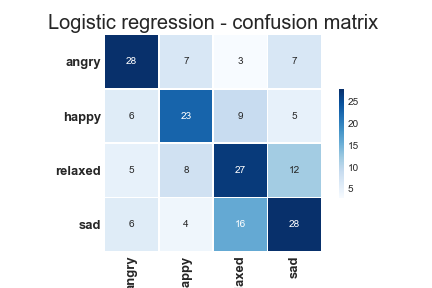
\includegraphics[width=\linewidth]{./chapters/chapter5/images/4Q/CM_LR.png}
    \caption{ML4Q}
  \end{subfigure}
  \begin{subfigure}[b]{0.49\linewidth}
   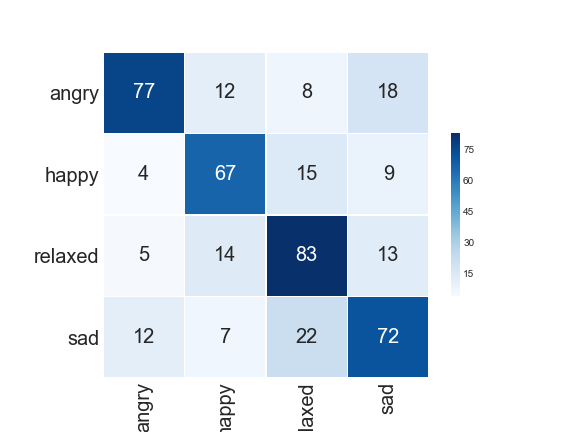
\includegraphics[width=\linewidth]{./chapters/chapter5/images/join/CM_LR.png}
    \caption{ML + ML4Q}
  \end{subfigure}
  \caption{Logistic Regression - Confusion Matrix}
  \label{fig:lr}
\end{figure}

\begin{figure}[H]
  \centering
  \begin{subfigure}[b]{0.49\linewidth}
    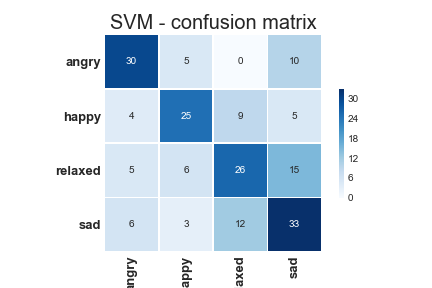
\includegraphics[width=\linewidth]{./chapters/chapter5/images/4Q/CM_SVM.png}
    \caption{ML4Q}
  \end{subfigure}
  \begin{subfigure}[b]{0.49\linewidth}
   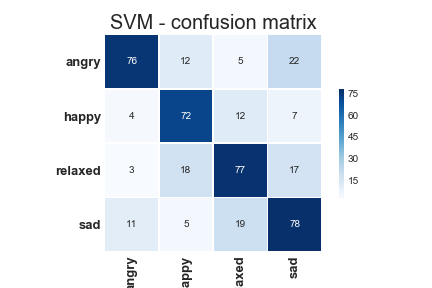
\includegraphics[width=\linewidth]{./chapters/chapter5/images/join/CM_SVM.png}
    \caption{ML + ML4Q}
  \end{subfigure}
  \caption{Support Vector Machine - Confusion Matrix}
  \label{fig:svm}
\end{figure}

\begin{figure}[H]
  \centering
  \begin{subfigure}[b]{0.49\linewidth}
    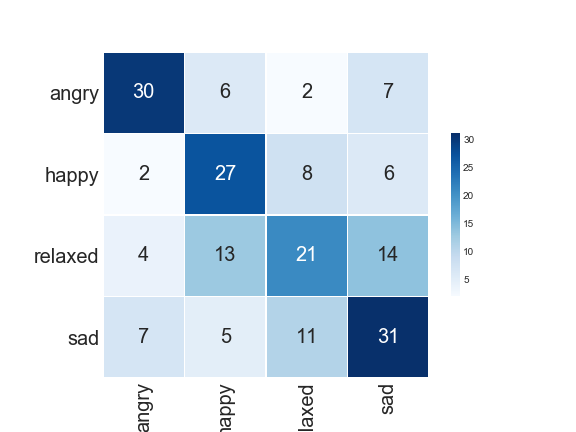
\includegraphics[width=\linewidth]{./chapters/chapter5/images/4Q/CM_XGB.png}
    \caption{ML4Q}
  \end{subfigure}
  \begin{subfigure}[b]{0.49\linewidth}
   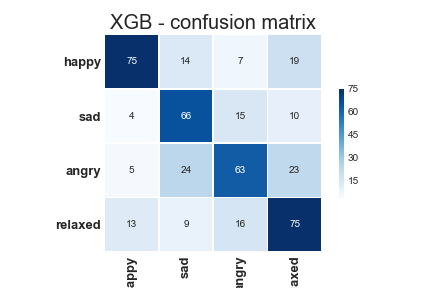
\includegraphics[width=\linewidth]{./chapters/chapter5/images/join/CM_XGB.png}
    \caption{ML + ML4Q}
  \end{subfigure}
  \caption{Xgboost - Confusion Matrix}
  \label{fig:xgb}
\end{figure}




